\documentclass[]{article}
\usepackage{ifxetex,ifluatex}
\ifnum 0\ifxetex 1\fi\ifluatex 1\fi=0 % if pdftex
\usepackage[T1]{fontenc}
\usepackage[utf8]{inputenc}
\usepackage[table,xcdraw]{xcolor}
\usepackage[margin=1.5in]{geometry}
\usepackage[tableposition=top]{caption}
\usepackage{tabularx}
\usepackage{hyperref}
\usepackage{graphicx}
\hypersetup{
colorlinks=true,
linkcolor=blue,
filecolor=magenta,
urlcolor=cyan,
}



\title{\textbf{Patients Transit Visualizer}\\Specyfikacja funkcjonalna projektu zespołowego}
\author{\small{AiSD GR2}\\Martyna Jakubowska, Hubert Nakielski, Artur Prasuła}
\date{Grudzień 2020}


\begin{document}
    \maketitle


    \section{Opis ogólny}

    \subsection{Nazwa programu}
    Patients Transit Visualizer

    \subsection{Poruszany problem}
    Program, na podstawie dostarczonych danych, ma za zadanie pomóc zespołowi ratowników z Karetek Pogotowia (KP) przewozić pacjentów (P) do Ośrodków Medycznych (OM). Program dla każdego wprowadzonego pacjenta będzie wskazywał najbliższy w danej chwili pacjentowi Ośrodek Medyczny i symulował przetransportowanie go do wspomnianego obiektu do póki nie znajdzie wolnego miejsca lub nie odwiedzi wszystkich OM.

    \subsection{Użytkownik docelowy}
    Program dedykowany jest służbie zdrowia do planowania najbardziej optymalnych tras karetek.
    Użytkownikami programu będą dyspozytorzy, którzy wydają rozkazy co do tras karetek.


    \section{Opis funkcjonalności}

    \subsection{Jak korzystać z programu}
    Do uruchomienia programu użytkownik będzie musiał mieć zainstalowane środowisko \textbf{Java 14} na swoim komputerze.
    Aby uruchomić program należy dwukrotnie nacisnąć ikonę pliku .jar. Następnie pojawi się okno, w którym należy wczytać plik zawierający dane do przeprowadzenia symulacji.

    \subsection{Możliwości programu}
    \begin{enumerate}
        \item Wczytanie informacji o szpitalach, obiektach i drogach z pliku tekstowego.
        \item Wczytanie listy pacjentów do obsługi z pliku tekstowego.
        \item Wykrycie błędów w plikach wejściowych i poinformowanie użytkownika o nich.
        \item Wczytanie nowego pacjenta do obsługi z poziomu GUI.
        \item Wizualizacja planszy wraz ze szpitalami, obiektami, drogami i skrzyżowaniami.
        \item Przeprowadzenie symulacji obsługi pacjentów i wyświetlenie jej przebiegu.
        \item Poinformowanie użytkownika o przesyceniu szpitali.
        \item Obliczanie współrzędnych skrzyżowań na podstawie danych wczytanych z pliku wejściowego.
        \item Obliczanie granic kraju.
    \end{enumerate}
    


    \section{Format danych i struktura plików}

    \subsection{Struktura katalogów}
    \textcolor{orange}{Proj\_zesp\_AiSD\_2020Z\_GR1}

    |---\textcolor{orange}{src}

    |\hspace{4mm} |-----\textcolor{orange}{ptv}

    |\hspace{15mm}|-----\textcolor{orange}{models} - \textit{przechowuje wszystkie obiekty związane z logiką programu}

    |\hspace{15mm}|-----\textcolor{orange}{views} -\textit{ odpowiada za wizualizację mapy i poszczególnych przewozów}

    |\hspace{15mm}|-----\textcolor{orange}{controllers} -\textit{ zajmuje się obsługą żądań użytkownika}

    |

    |

    |---\textcolor{orange}{test}

    \hspace{5mm} |-----\textcolor{orange}{ptv}

    \hspace{16mm}|-----\textcolor{orange}{models}

    \hspace{16mm}|-----\textcolor{orange}{controllers}

    \subsection{Przechowywanie danych w programie}
    Dane wejściowe są przechowywane w listach (ArrayList) zawierających poszczególne obiekty. \\
    Każdy Ośrodek Medyczny (OM) reprezentowany jest przez obiekt typu\textit{ Hospital}, a wszystkie obiekty tego typu gromadzone są w liście. Dodatkowo OM zawiera listę dróg \textit{(Distance}) do innych, niekoniecznie wszystkich, OM.\\
    Obiekty (tj. pomniki, muzea, \ldots) przechowywane są w liście zawierającej obiekty typu \textit{Facility}.\\
    Pacjenci, reprezentowani przez obiekt \textit{Patient}, również przechowywani są w liście.\\

    Klasy obiektów i reprezentowane w nich dane:\\


    \textit{Hospital}
    \begin{itemize}
        \item  \textcolor{gray}{int} id
        \item  \textcolor{gray}{String} nazwa
        \item  \textcolor{gray}{double} współczynnik x
        \item \textcolor{gray}{double}  współczynnik y
        \item \textcolor{gray}{int}  liczba wszystkich łóżek
        \item \textcolor{gray}{int}  liczba dostępnych łóżek
    \end{itemize}

    \textit{Facility}
    \begin{itemize}
        \item  \textcolor{gray}{int} id
        \item  \textcolor{gray}{String}  nazwa
        \item  \textcolor{gray}{double}  współczynnik x
        \item \textcolor{gray}{double}  współczynnik y
    \end{itemize}

    \textit{Distance}
    \begin{itemize}
        \item \textcolor{gray}{int}  id
        \item  \textcolor{gray}{int} id pierwszego OM |
        \item  \textcolor{gray}{int} id drugiego OM |
        \item \textcolor{gray}{double}  odległość (jednostka reprezentująca czas)
    \end{itemize}

    \textit{Patient}
    \begin{itemize}
        \item  \textcolor{gray}{int} id
        \item \textcolor{gray}{double}  współczynnik x
        \item \textcolor{gray}{double}  współczynnik y
    \end{itemize}

    \subsection{Dane wejściowe}
    Do programu będzie można przekazać dwa pliki tekstowe. Plik z danymi o szpitalach, obiektach i drogach oraz plik z listą pacjentów do obsługi. \\
    \\
    Wzór pliku z danymi o szpitalach, obiektach i drogach: \\
    \textcolor{gray}{\# Szpitale} \\
    id | nazwa | wsp. x | wsp. y | liczba łóżek | liczba wolnych łóżek \\
    \textcolor{gray}{\# Obiekty} \\
    id | nazwa | wsp. x | wsp. y \\
    \textcolor{gray}{\# Drogi} \\
    id | id szpitala | id szpitala | odległość \\
    \\
    Wzór pliku z listą pacjentów do obsługi: \\
    \textcolor{gray}{\# Pacjenci} \\
    id | wsp. x | wsp.y \\
    \\
    Opis poszczególnych sekcji: \\
    \textbf{id} - numer identyfikacyjny, unikalna i nieujemna liczba całkowita mniejsza od 1000. \\
    \textbf{nazwa} - nazwa szpitala lub obiektu, unikalny ciąg znaków nie zawierający znaku ,,|'' \\
    \textbf{wsp. x} - współrzędna x szpitala lub obiektu na mapie, liczba całkowita lub zmiennoprzecinkowa \\
    \textbf{wsp. y} - współrzędna y szpitala lub obiektu na mapie, liczba całkowita lub zmiennoprzecinkowa \\
    \textbf{liczba łóżek} - liczba wszystkich łóżek w szpitalu, suma zajętych i dostępnych łóżek, całkowita i nieujemna liczba całkowita \\
    \textbf{liczba wolnych łóżek} - liczba łóżek, które są wolne w szpitalu, całkowita i nieujemna liczba całkowita \\
    \textbf{id szpitala} - numer identyfikacyjny szpitala, który jest połączony daną drogą, szpital o takim \textbf{id} musi zostać wcześniej wczytany \\
    \textbf{odległość} - długość drogi łączącej dwa szpitale, nieujemna liczba całkowita lub zmiennoprzecinkowa \\
    \\
    Jeśli położenie pacjenta, będzie poza granicami państwa (granice państwa są wyznaczane jako najmniejszy zbiór wypukły zawierający wszystkie szpitale i obiekty) pacjent nie zostanie obsłużony.
    Plik nie może zawierać kilku takich samych szpitali/obiektów/dróg/pacjentów.
    Każda z sekcji w jednym ze szpitali/obiektów/dróg/pacjentów musi zostać oddzielona separatorem ,,|''.
    Sekcje w których wypisujemy szpitale/obiekty/drogi, w pliku zawierającym te dane, powinny być w odpowiedniej kolejności: szpitale, obiekty, drogi.
    Sekcje te dodatkowo powinny zostać oddzielone linią w której pierwszy znak to ,,\#''.
    Plik tekstowy z listą pacjentów nie musi zawierać linii zaczynającej się od ,,\#'' (takie linie będą ignorowane przez program).
    Puste linie w plikach obu wejściowych będą ignorowane przez program. \\
    \\
    Przykładowy plik wejściowy zawierający szpitale. obiekty i drogi. \\
    \\
    \textcolor{gray}{\# Szpitale (id | nazwa | wsp. x | wsp. y | Liczba łóżek | Liczba wolnych łóżek)} \\
    1 | Szpital Wojewódzki nr 997 | 10 | 10 | 1000 | 100 \\
    2 | Krakowski Szpital Kliniczny | 100 | 120 | 999 | 99 \\
    3 | Pierwszy Szpital im. Prezesa RP | 120 | 130 | 99 | 0 \\
    4 | Drugi Szpital im. Naczelnika RP | 10 | 140 | 70 | 1 \\
    5 | Trzeci Szpital im. Króla RP | 140 | 10 | 996 | 0 \\
    \\
    \textcolor{gray}{\# Obiekty (id | nazwa | wsp. x | wsp. y)} \\
    1 | Pomnik Wikipedii | -1 | 50 \\
    2 | Pomnik Fryderyka Chopina | 110 | 55 \\
    3 | Pomnik Anonimowego Przechodnia | 40 | 70 \\
    \\
    \textcolor{gray}{\# Drogi (id | id szpitala | id szpitala | odległość)} \\
    1 | 1 | 2 | 700 \\
    2 | 1 | 4 | 550 \\
    3 | 1 | 5 | 800 \\
    4 | 2 | 3 | 300 \\
    5 | 2 | 4 | 550 \\
    6 | 3 | 5 | 600 \\
    7 | 4 | 5 | 750 \\
    \\
    Przykładowy plik zawierający listę pacjentów do obsługi: \\
    \\
    \textcolor{gray}{\# Pacjenci (id | wsp. x | wsp.y)} \\
    1 | 20 | 20 \\
    2 | 99 | 105 \\
    3 | 23 | 40 \\
    
    \subsection{Dane wyjściowe}
    Program pokazuje wynik działania w graficznym interfejsie użytkownika w postaci przewiezionych pacjentów do wskazanych przez program OM lub komunikatu o brakujących wolnych miejscach w OM.


    \section{Scenariusz działania programu}

    \subsection{Scenariusz ogólny}
    \begin{enumerate}
        \item Uruchomienie programu
        \item Wczytanie pliku wejściowego zawierającego dane OM, obiektów oraz dróg
        \item Wizualizacja OM oraz obiektów na mapie
        \item Wczytanie listy pacjentów z pliku wejściowego, bądź dodanie pojedynczego pacjenta z poziomu graficznego poprzez odpowiedni formularz
        \item Symulacja obsługi pacjentów
        \item Zakończenie programu
    \end{enumerate}

    \subsection{Scenariusz szczegółowy}
    \begin{enumerate}
        \item[1.] Uruchomienie programu.
        \item[2.] Wczytanie pliku wejściowego zawierającego dane OM, obiektów oraz dróg.
            \subitem[2.1.] Wczytanie nastąpi po naciśnięciu odpowiedniego przycisku i wybraniu pliku z okna dialogowego.
            \subitem[2.2.] W przypadku próby wczytania niepoprawnego pliku, program nie wczyta go i poinformuje użytkownika o napotkanym błędzie.
        \item[3.] Wizualizacja OM oraz obiektów na mapie.
            \subitem[3.1.] Obliczenie współrzędnych skrzyżowań na podstawie wczytanych dróg.
            \subitem[3.2.] Wyświetlenie szpitali, obiektów, dróg i skrzyżowań.
        \item[4.] Wczytanie listy pacjentów z pliku wejściowego, bądź dodanie pojedynczego pacjenta z poziomu graficznego poprzez odpowiedni formularz.
            \subitem[4.1.] Wczytanie nastąpi po naciśnięciu odpowiedniego przycisku i wybraniu pliku z okna dialogowego.
            \subitem[4.2.] W przypadku próby wczytania niepoprawnego pliku, program nie wczyta go i poinformuje użytkownika o napotkanym błędzie.
        \item [5.]Symulacja obsługi pacjentów.
            \subitem[5.1.] Wczytanie nastąpi po naciśnięciu odpowiedniego przycisku.
            \subitem[5.2.] Symulacja wykona się z określoną przez użytkownika szybkością.
            \subitem[5.3.] W przypadku próby obsługi pacjenta poza granicami państwa, program wypisze odpowiedni komunikat i pominie tego pacjenta.
            \subitem[5.4.] W przypadku przepełnienia ośrodków medycznych, program wyświetli odpowiedni komunikat.
        \item[6.] Zakończenie programu.
    \end{enumerate}
        
    \subsection{Ekrany działania programu}
    \begin{figure}[!h]
    \centering
    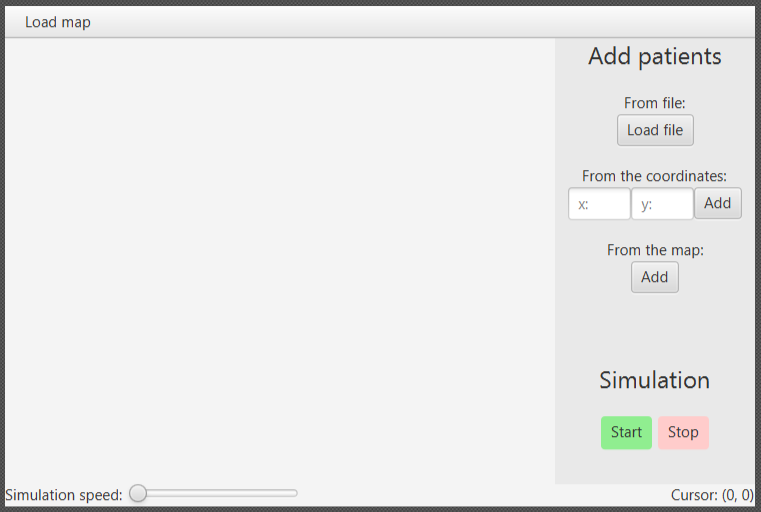
\includegraphics[width=\textwidth]{gui.jpg}
    \caption{Ekran działania programu}
    \label{fig:Shrek}
    \end{figure}
    Ekran działania programu służy do załadowania mapy, następnie wczytywania pacjentów oraz kontrolowania symulacji. GUI jest podzielone na następujące sekcje:
    \begin{itemize}
    \item menu górne, gdzie znajduje się przycisk 'Load map' służy do wczytania pliku tekstowego z danymi szpitali, obiektów i dróg.
    \item menu boczne, podzielone na 2 działy: 
    \begin{itemize}
    \item 'Add patients' - służy do dodawania pacjentów (po wczytaniu mapy), za pomcą pliku tekstowego, wpisania współżędnych lub poprzez naciśnięcie odpowiedniego punktu na mapie
    \item 'Simulation' - służy do kontrolowania symulacji, po wczytaniu mapy i dodaniu pacjentów możemy rozpoczynać i zatrzymywać oraz wznawiać proces
    \end{itemize}
    \item pasek boczny - po lewej stronie znajduje się suwak do ustawiania prędkości symulacji, po prawej funkcja 'Cursor', która pokazuje na jakiej współrzędnej na mapie znajduje się obecnie kursor 
    \end{itemize}


    \section{Testowanie}
    Poszczególne klasy programu zostaną przetestowane za pomocą testów jednostkowych. Do tego posłuży nam narzędzie JUnit. Współpraca klas w programie oraz działanie graficznego interfejsu użytkownika zostanie przetestowane przez nas ręcznie w trakcie implementacji.

\end{document}